\documentclass{standalone}
\usepackage{tikz}
\begin{document}
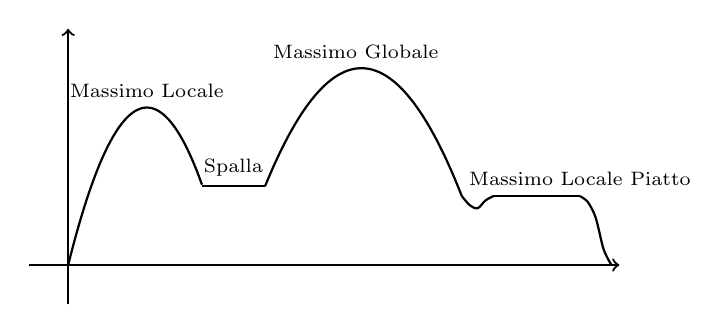
\begin{tikzpicture}[scale=2]
    \draw[->, thick](-0.25,0)--(3.5,0);
    \draw[->, thick](0,-0.25)--(0,1.5);
    \draw[thick]plot[smooth, domain=0:0.85](\x, {-((\x-1/2)*2)^2+1});
    \draw[thick](0.85,0.5)--(1.25,0.5)node[midway, above]{\scriptsize Spalla};
    \draw[thick]plot[smooth, domain=1.25:2.5](\x,{-0.5*((\x-3.725/2)*2)^2+1.25});
    \draw 
    (0.5,1)node[above]{\scriptsize Massimo Locale}
    (1.8265, 1.25)node[above]{\scriptsize Massimo Globale}
    ;
    \draw[thick](2.7,0.43719)--++(0.55,0)node[above]{\scriptsize Massimo Locale Piatto};
    \draw[thick]plot[smooth]coordinates{(2.5,0.43719) (2.55,0.38) (2.6,0.36) (2.65,0.41) (2.7,0.43719)};
    \draw[thick]plot[smooth]coordinates{(3.25,0.43719) (3.3, 0.4) (3.35, 0.3) (3.4, 0.1) (3.45, 0)};
\end{tikzpicture}
\end{document}